\section{Introduction}
\label{sec:intro}

Creating a Geant4 simulation application devoid of hardcoded numbers can be achieved
by replacing conventional calls like ~\verb|G4Box(‘box’, 20, 30, 40)| with
code like~\verb|G4Box(name, a, b, c)| where the parameters are sourced from a database.
This however does not eliminate the need for users to write in C++ and Geant4 code
and engage in the essential tasks of organizing the volumes, specify sensitivities,
formulating the digitization of Geant4 steps, and collecting and saving the resulting hits.


\begin{figure}[h]
    \centering
    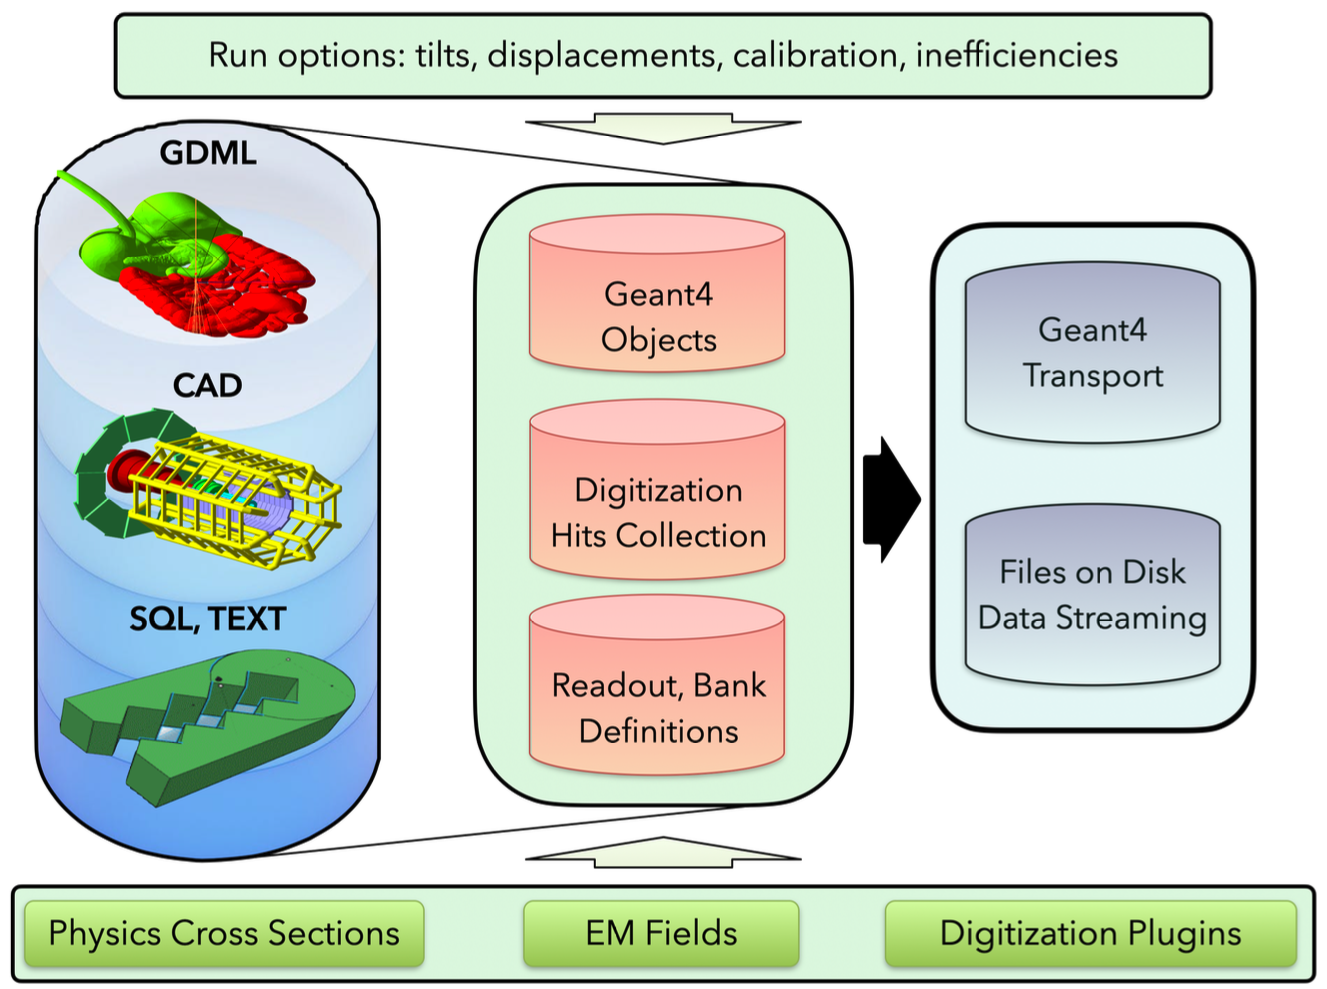
\includegraphics[width=.95\textwidth]{img/db}
    \caption{GEMC: a Geant4 application driven in its entirety by databases: geometry, materials,
        digitization, readout electronics, output format. Additional configurations such as which phusics
        list to use, magnetic field, which experment to run can be provided by steering cards (JSON).}
    \label{fig:db}
\end{figure}

An application such as the one sketched Fig.\ref{fig:db}, capable of driving in its entirety
a Geant4 simulation from databases and steering cards present several advantages:

\begin{itemize}
    \item No need for prior expertise in C++ or Geant4.
    \item The focus squarely shifts towards
    the geometry aspect, facilitated by seamless interactions with databases,
    allowing users to concentrate on experiment-specific details without the burden of coding intricacies.
    \item The experiment setup is effortlessly shared without necessitating code recompilation.
    This agility enhances teamwork, limits debugging and accelerates development.
    \item It serves as a unified platform capable of simulating diverse experiments.
    Users can readily switch between experiments by selecting their desired configurations from the database.
\end{itemize}

\newpage
We present the database driven GEMC\cite{clas12_gemc, gemc_homepage}, a versatile solution that offers:

\begin{itemize}
    \item Intuitive Python API: GEMC empowers users with an accessible Python API, enabling
    effortless detector construction and seamless database population.
    Additionally, it supports CAD (STL) and GDML imports, further simplifying the setup process.
    \item Hardware Emulation: GEMC incorporates hardware emulation for readout electronics.
    This allows users to mimic real-world electronic components, enhancing the accuracy and realism of
    the simulations.
    \item Custom Digitization: the flexibility to define custom digitization procedures for Geant4 steps
    ensures that simulations align precisely with specific experimental requirements.
    \item Data Streaming: downstream analysis is facilitated by the options to stream simulation results directly
    to disk or network storage.
    Pre-loaded plugins provide ROOT and TEXT output formats.
\end{itemize}


\section{Features}
\label{sec:features}

\subsection{Geometry Sources}
\label{subsec:databases}
GEMC offers multiple sources for reading geometry and materials definitions,

\begin{itemize}
    \item CAD Import (STL): Objects are defined using STL files, loaded via
    steering cards.
    Optional JSON files can add attributes like materials,
    hierarchy, position, rotation, etc.
    \item GDML files: same as CAD import, but the geometry is defined
    in a GDML file.
    \item Databases and Text Files: Native Geant4 geometry and materials can be defined
    using Python API and stored in databases (MySQL, Sqlite) or text files.
    This includes combining volumes through copy and boolean operations.
\end{itemize}
Users may define volume hierarchies mixing sources.
For instance, a CAD file can be imported and serve as the parent for a volume
defined in a database, or vice versa.
This versatility empowers users to create complex geometries with ease.

\subsection{Python API}
\label{subsec:api}
Designed with a user-centric approach, the API prioritizes intuition and simplicity,
requiring no additional code beyond its usage to develop a comprehensive simulation.

In Fig.\ref{fig:api} the code to build a cylindrical target and
a sensitive ``flux'' detector is shown.

\begin{figure}[h]
    \centering
    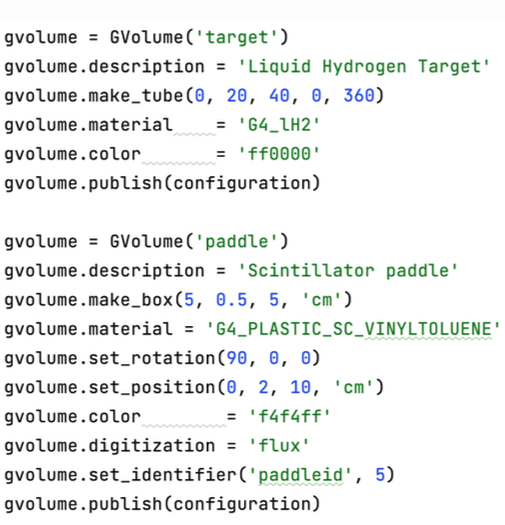
\includegraphics[width=.40\textwidth]{img/api_snippet}
    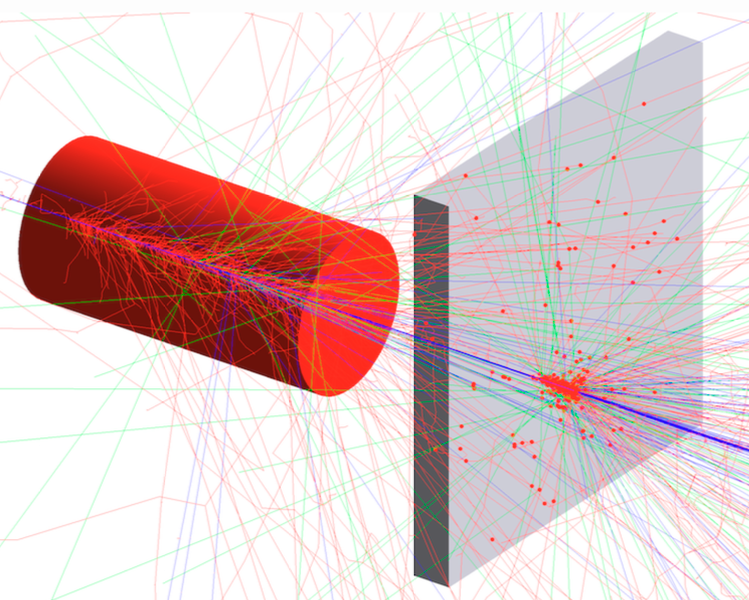
\includegraphics[width=.58\textwidth]{img/api}
    \caption{An example demonstrating the simplicity of the Python API to build a detector and populate the databases:
    Left: the code snippet creates a cylindrical target and a sensitive flux box scintillator.
    Notice how users need only to fill entries with
    quantities they are familiar with, such as shape type, dimensions, etc, and not
    worry about the code necessary to define the geant4 objects, assign sensitivity to the
    scintillator, collect hits and writing the output.
    Right: the resulting geometry. The flux scintillator paddle collects hits from proton
    impinging on the liquid hydrogen target.}
    \label{fig:api}
\end{figure}

\subsection{Electronic Time Window and Energy Sharing}
\label{subsec:time_window}

Replicating the data collection mechanism is essential to ensure that a simulation is
indistinguishable from real experimental data.
In GEMC, this crucial aspect is seamlessly integrated for all sensitive detectors,
simplifying the process for users.

The collection of digitized values, such as integers (ADC, TDC)
or payloads (FADC), within a user-set time window is handled automatically by GEMC,
see Fig.\ref{fig:time_window_energy_sharing} (left).

Furthermore, GEMC offers the capability to artificially generate hits, mimicking the phenomenon of
energy sharing commonly observed in real detectors, especially among adjacent sensitive elements like silicon strips.
The realism of simulations is enhanced by simulating energy distribution and sharing patterns
that occur naturally in experimental setups, see for example Fig.\ref{fig:time_window_energy_sharing} (right).

\begin{figure}[h]
    \centering
    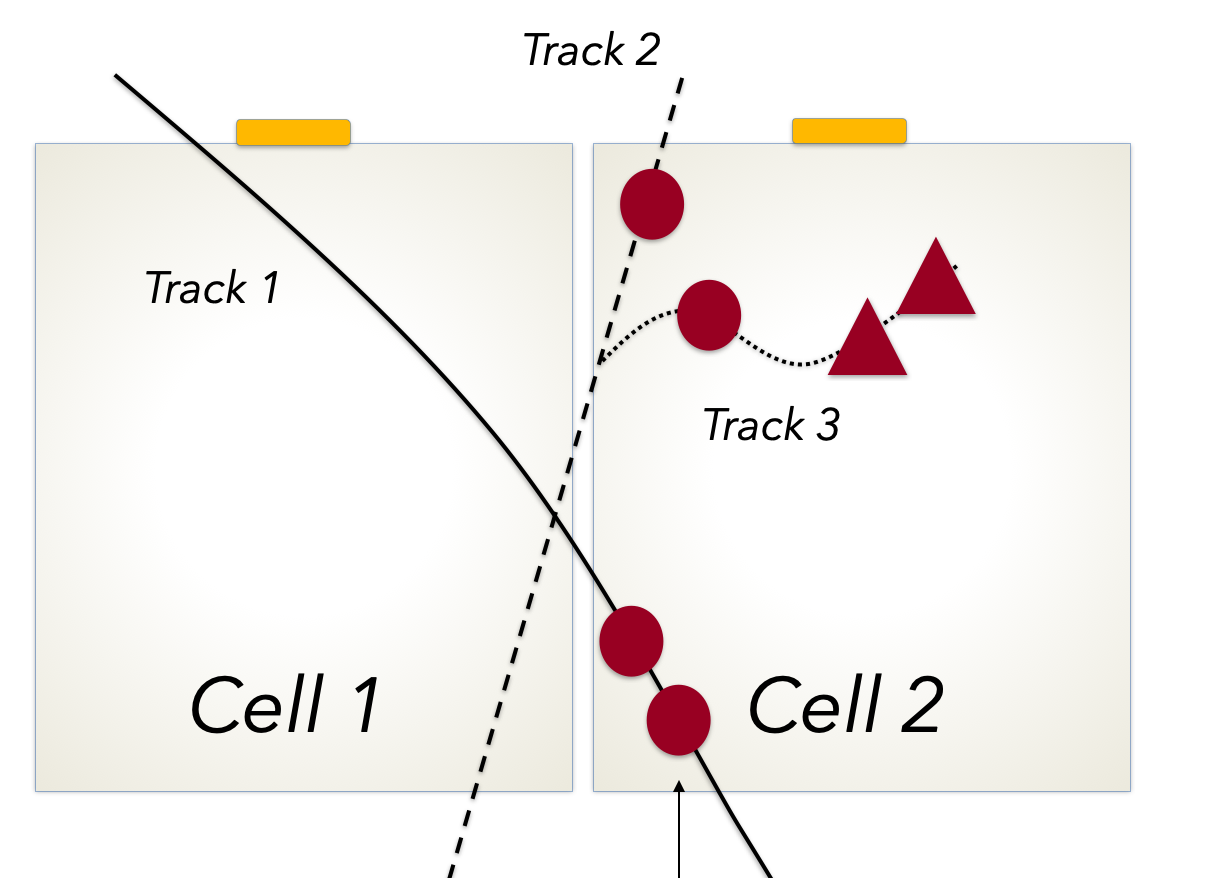
\includegraphics[width=.45\textwidth]{img/tw}
    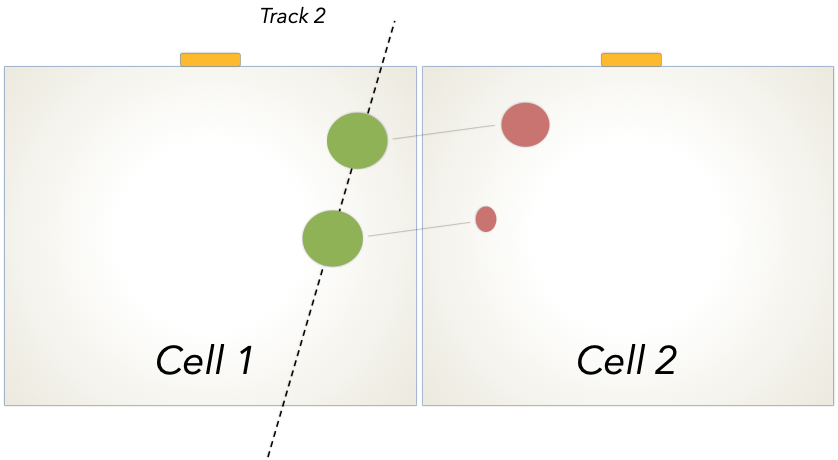
\includegraphics[width=.54\textwidth]{img/e_sharing}
    \caption{Left: in this scenario, two primary tracks and a secondary track deposit energy within
    the sensitive element ``cell 2''. The triangular steps associated with the secondary track
    exhibit a significant time difference compared to the circular steps, exceeding the sensitive time window
    As a result, GEMC correctly produces two separate hits, collecting the circles into one and the triangles
    in the other one, mirroring the behavior of realistic readout electronics.
    Right: the Geant4 steps are shown in green. The red steps are artificially generated
    by GEMC, with a user-defined algorithm, to mimic energy sharing.
    Energy sharing among adjacent sensitive elements is a common phenomenon in real detectors.}
    \label{fig:time_window_energy_sharing}
\end{figure}

\subsection{Sensitivity and Digitization}
\label{subsec:digitization}

The digitization of Geant4 steps is a pivotal aspect of the simulation process.
GEMC simplifies this critical step by offering an intuitive interface that presents Geant4 steps
with commonly used algorithms.
Here is an overview of the functionalities it supports:

\begin{itemize}
    \item Readout Electronics Parameters: define parameters such as the time window,
    aligning simulations with real-world data acquisition.
    \item Energy Sharing and Hit Proliferation: customize energy sharing and hit proliferation mechanism.
    \item Calibration and Digitization Constants: Load parameters from databases sources.
    \item Translation Table: map Geant4 volume identifiers to crate/slot/channel
    \item Hit Digitization: collection and treatment of Geant4 steps
    \item Streaming Readout: Define parameters for data streaming to disk or network storage.
    \item Output Bank: Specify the output organization for hits, such as ADC, TDC, FADC, or SRO payload.
\end{itemize}

GEMC's plugin framework streamlines the digitization process, allowing users to tailor simulations
to closely match real-world data acquisition systems while maintaining flexibility and ease of use.

\subsection{Data Streamer}
\label{subsec:data_streamer}

GEMC provides Data Streamers to handle the storage of data to files or disk.
These streamers are stored in dynamic libraries, separate from the GEMC core, ensuring modularity
and maintainability and allowing users to create their own streamers.

They offer structured access to data collection classes like GEventDataCollection (for event-by-event hits)
and GFrameDataCollection (for time-based hits).
These streamers support a wide array of formats, including general ones like TEXT and ROOT,
as well as Jefferson Lab-specific formats like HIPO, EVIO, and VTP Binary.
This workflow simplifies data publishing, allowing users to concentrate solely on defining the variables to be
added to the data collection without concerning themselves with the intricacies of the output format.

\section{Examples}
\label{sec:examples}

Two GEMC examples that showcase its versatility and practicality are shown.
The first illustrates the Computer-Aided Design (CAD) integration.
The second example takes us to the CLAS12 experiment at Jefferson Lab, where GEMC plays the role
of simulating and calculating the response of real-world experiments and data acquisition processes.
These illustrations underscore GEMC's contribution to simplifying simulation tasks,
empowering researchers to focus on their scientific pursuits.

\subsection{Cad Import}
\label{subsec:cad_import}

This example highlights GEMC's versatility in handling CAD imports and its ability to create engaging
simulations of complex scenarios with minimal coding.
The goal is to visualize and simulate interactions between two iconic spacecraft: an Enterprise ship and a Romulan ship.

The volumes are imported directly from two \emph{Stereolithography (STL)}\footnote{STL: A widely used file format
in 3D computer-aided design (CAD) and 3D printing. STL represents 3D surfaces as a collection of interconnected triangles}
files: ``enterprise.stl'' and ``romulan.stl''.
The following line in a JSON steering card takes care of the romulan ship color, including its transparency that honors the cloaking technology,
and assigns the ``flux'' sensitivity to it:

\begin{verbatim}
"romulans": {"color": "ff99bb4", "digitization": "flux"}
\end{verbatim}


No actual code is required to run the simulation,  shown in Fig.\ref{fig:cad_import}.



\begin{figure}[h]
    \centering
    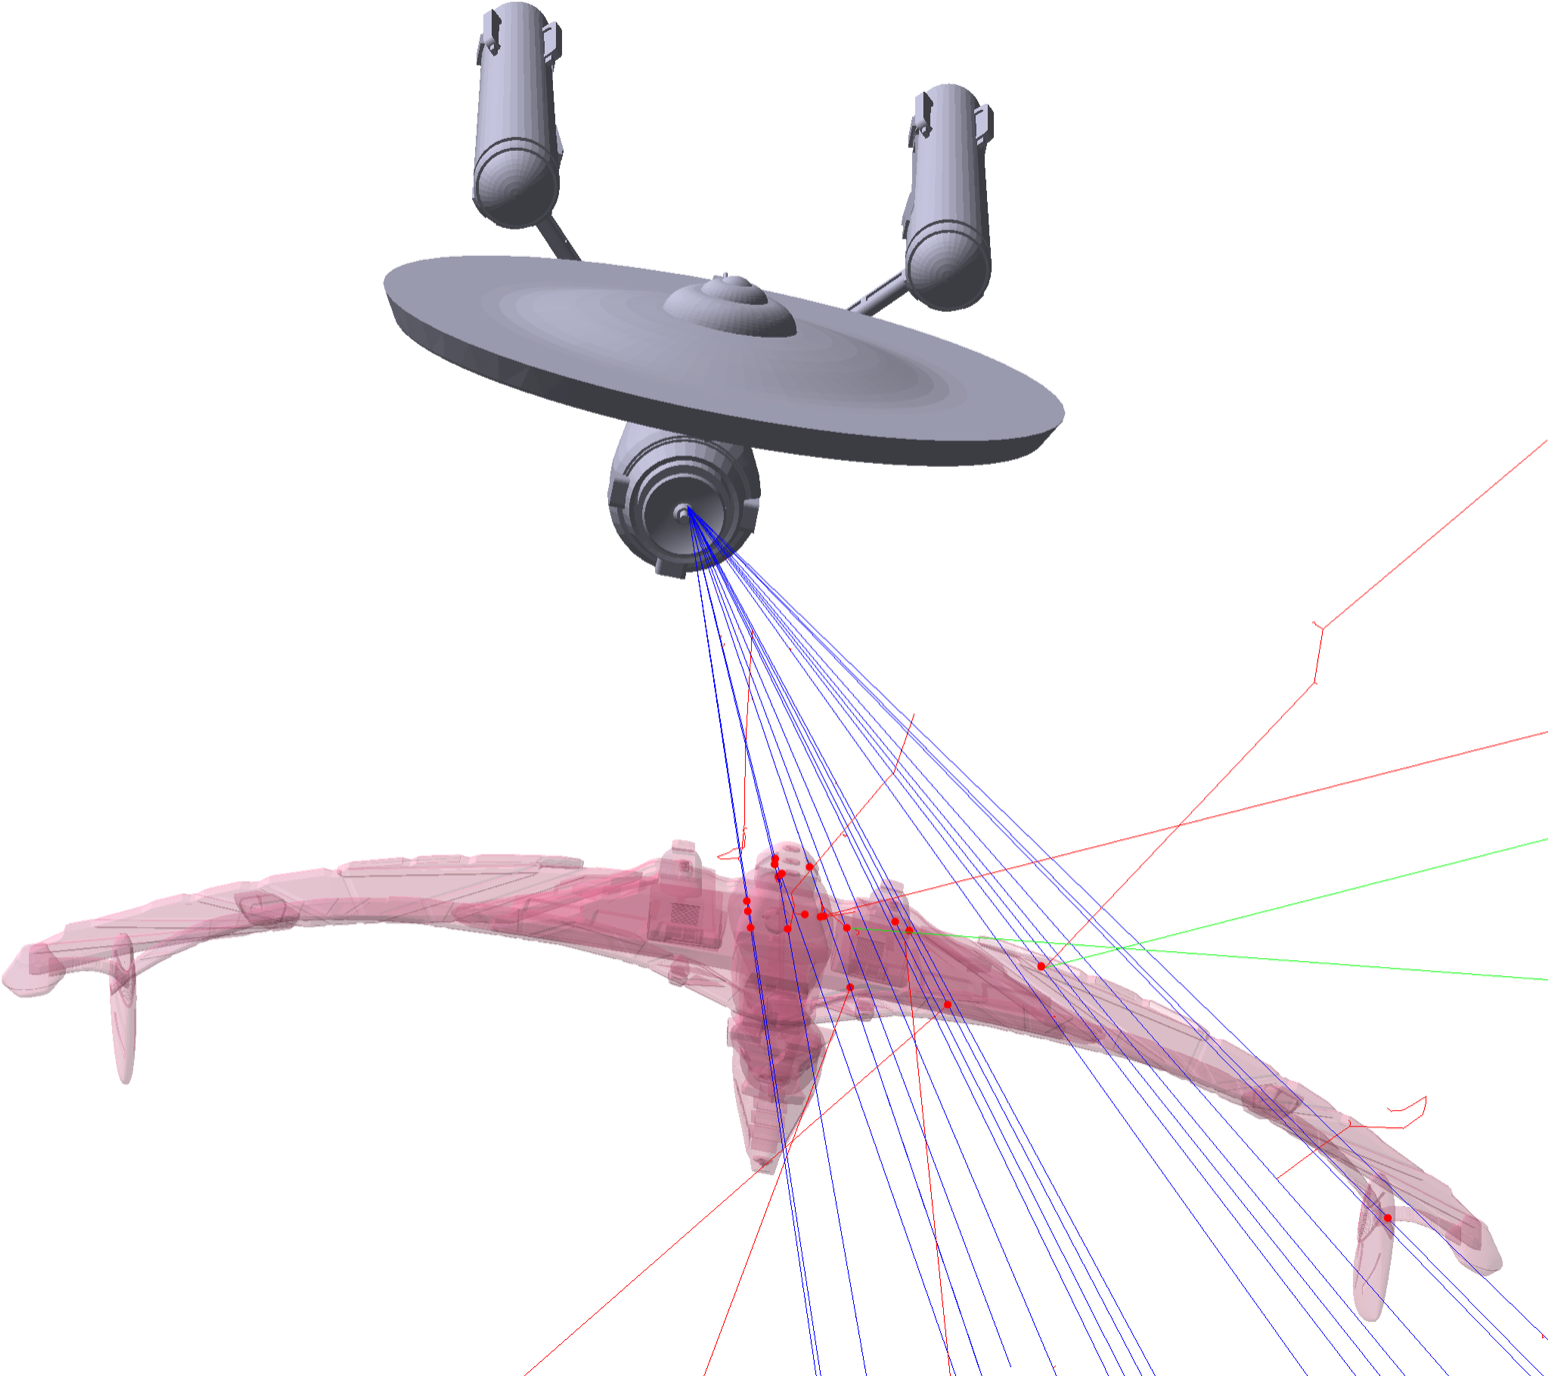
\includegraphics[width=.5\textwidth]{img/startrek}
    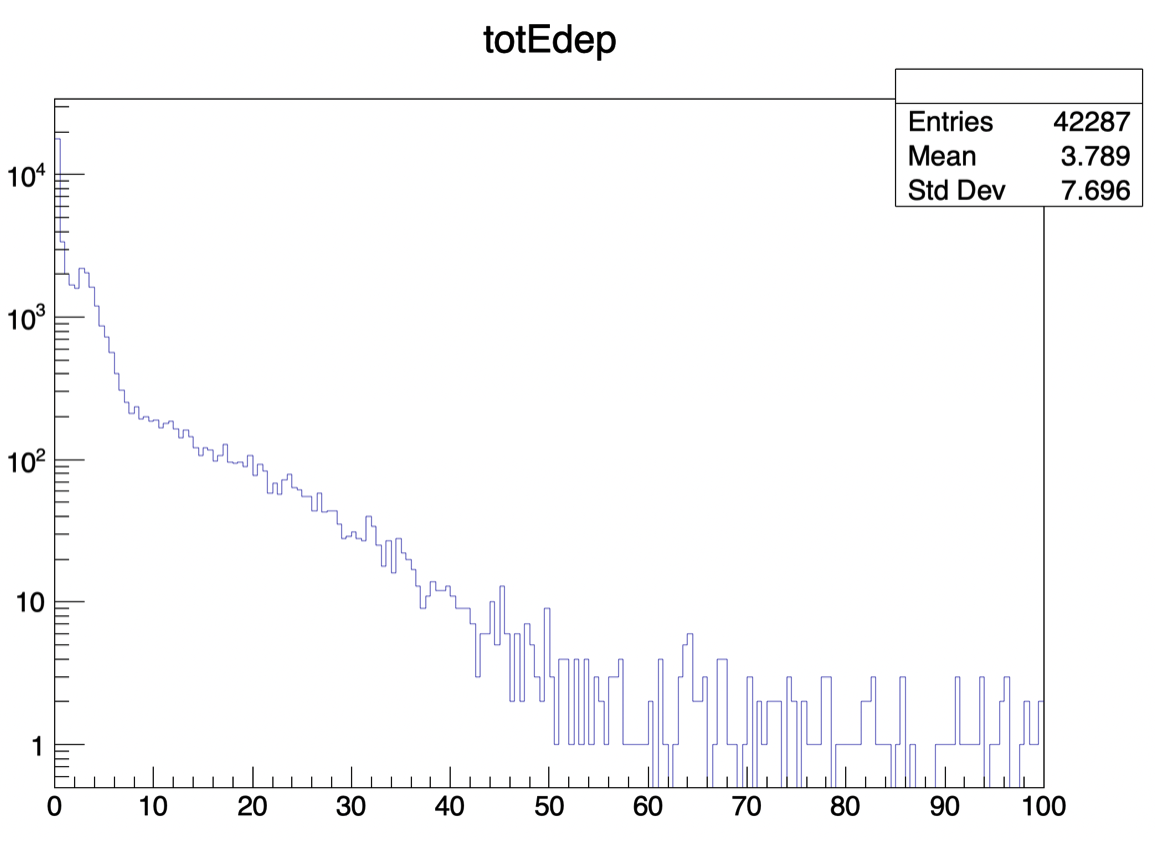
\includegraphics[width=.48\textwidth]{img/startrek_edep}
    \caption{Left: the geometry of the Enterprise and Romulan ships imported from STL files.
    The Romulan ship is assigned the ``flux'' sensitivity and a color, including transparency, via a single line in a JSON steering card.
    With command line options a proton beam is shot at the Romulan ship.
    Right: the plot of energy deposited in the Romulan ship.}
    \label{fig:cad_import}
\end{figure}


\subsection{GEMC at Jefferson Lab}
\label{subsec:clas12}


\section{Summary}
\label{sec:summary}

